\documentclass[xcolor={dvipsnames}]{beamer}
%  \usetheme{JuanLesPins}
   \usetheme{Boadilla}
%   \setbeamertemplate{frametitle continuation}[from second]
%   \setbeamertemplate{bibliography entry title}{}
%   \setbeamertemplate{bibliography entry location}{}
%   \setbeamertemplate{bibliography entry note}{}
\usepackage[utf8]{inputenc}
\usepackage[english]{babel}
\usepackage{alltt}
\usepackage{graphicx}

%\usepackage{etex}
%\usepackage{ulem}
%\usepackage[all]{xy}
%\usepackage{tikz}
%\normalem
%\usepackage{alltt}
%\usepackage{fancyvrb}
%\usepackage{hyperref}
%\usepackage{pdfpages}
%\usepackage{comment}
\usepackage{booktabs}
%
%\usepackage{listings}
%\usepackage{algorithmic}
%\usepackage{datatool}
%
%
%%\usepackage{mathpartir}
%\usepackage{algorithmic}
%\usepackage{wasysym}

%\input{macros}

%\graphicspath{{pics/}{pics/logos/}} % Root directory of the pictures

%\input{macros}

\newcommand{\ZZZ}[1]{\textcolor{red}{#1}}
\newcommand{\EEE}[1]{\textcolor{BlueViolet}{#1}}

\title[Comigrate]%
{Comigrate: \\ improving package migration \\
 from \texttt{unstable} to \texttt{testing}}

\author[Di Cosmo/Dogguy/Vouillon]{Mehdi Dogguy, J\'er\^ome Vouillon and Roberto Di Cosmo}

\date[2014-01-18]{January 18, 2014}

\begin{document}

\begin{frame}[label=title]{}
 \titlepage
 \vspace{-1.5cm}
 \begin{center}
%  
\includegraphics[width=1cm]{p7} \hfill
%  
\includegraphics[width=2.5cm]{inria-logo-new} \hfill
%  
\includegraphics[width=2.5cm]{Logotype-IRILL} \hfill
%  
\includegraphics[width=1.5cm]{cnrsfilaire_quadri} \hfill
 \end{center}
\end{frame}

\part{Package migration}
\frame{\partpage}

\begin{frame}{Package Migration}

\begin{center}
\includegraphics[width=0.7\linewidth]{figures/migration}
\end{center}

\vspace{-1em}
\EEE{Conflicting goals}
\begin{itemize}
\item package should reach \textit{testing} rapidly
\item keep \textit{testing} as stable as possible
\end{itemize}

\end{frame}

\begin{frame}{Conditions for migration}
\EEE{Simple constraints} % (Boolean constraints):
\begin{itemize}
\item old enough
\item no new critical bug
\item simultaneous migration of source and binary packages
\item ...
\end{itemize}
\EEE{Complex constraints}
\begin{itemize}
\item packages should remain installable
\item (packages should remain co-installable)
\end{itemize}
\end{frame}

\begin{frame}[fragile]{Britney}
Shortcomings of Britney:
\begin{itemize}
\item Can fail to migrate automatically some packages
\item Hard do debug complex simultaneous migrations
\item Blind to co-installability issues
\end{itemize}

\begin{itemize}
\item need help
\begin{itemize}
\item many packages that have to migrate simultaneously 
\item smooth upgrade
\begin{quote}
\begin{verbatim}
trying: apr-util
skipped: apr-util (801 <- 513)
    got: 3+0: i-3
    * i386: libaprutil1-dbd-freetds
\end{verbatim}
\end{quote}
\end{itemize}
\item
blind to some issues: freebsd kernel, HDF mess, ...
(end user point of view...)

icedove migrating without enigmail, ...
\end{itemize}

I have about 200 packages that I know should migrate simultaneously.
How do I find which they are, why they don't migrate automatically
(bugs, broken dependencies, not old enough, ...)
\end{frame}

\begin{frame}{Co-installability issues}

Bug \#726517 \hspace{1cm}  enigmail: uninstallable in jessie due to FTBFS
\begin{quote}
the current version of enigmail in sid won’t migrate to jessie
because of an FTBFS (on kfreebsd). A version of icedove which
is incompatible with the old version of enigmail migrated to
jessie today.
\end{quote}

\end{frame}

\begin{frame}{libhfd5 in testing...}

\texttt{libhdf5-7} conflicts with \texttt{libhdf5-openmpi-7}

\textbf{Depend on libhdf5-openmpi-7:} libmed1 libpetsc3.2
libmedimport0 libsilo-bin libxdmf-dev libhdf5-mpi-dev libmedc1
libslepc3.2-dbg code-saturne libpetsc3.2-dev libsiloh5-0
code-saturne-include libmedc-dev libslepc3.2 libpetsc3.2-dbg
libsilo-dev libxdmf2 libmed-dev libmedimport-dev libslepc3.2-dev
syrthes code-saturne-bin petsc-dev python-silo fenics libmed-tools

\textbf{Depend on libhdf5-7:} libmapnik-dev libhe5-hdfeos-dev
grass-dev libmapnik2-dev liblas-dev libgdal-dev libqgis-dev
libhdfeos5-ruby1.8 libgdal1-dev
\end{frame}

\begin{frame}
\texttt{tesseract-ocr} incompatible with \texttt{tesseract-ocr-en}
\begin{center}
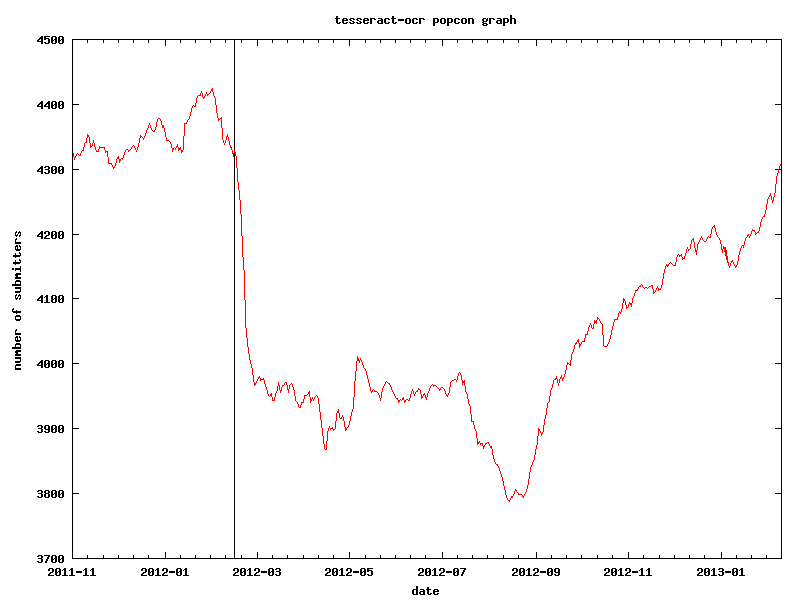
\includegraphics[width=0.8\linewidth]{figures/tesseract-ocr}
\end{center}
\end{frame}

\begin{frame}
\texttt{openclipart-libreoffice} incompatible with \texttt{libreoffice}
\begin{center}
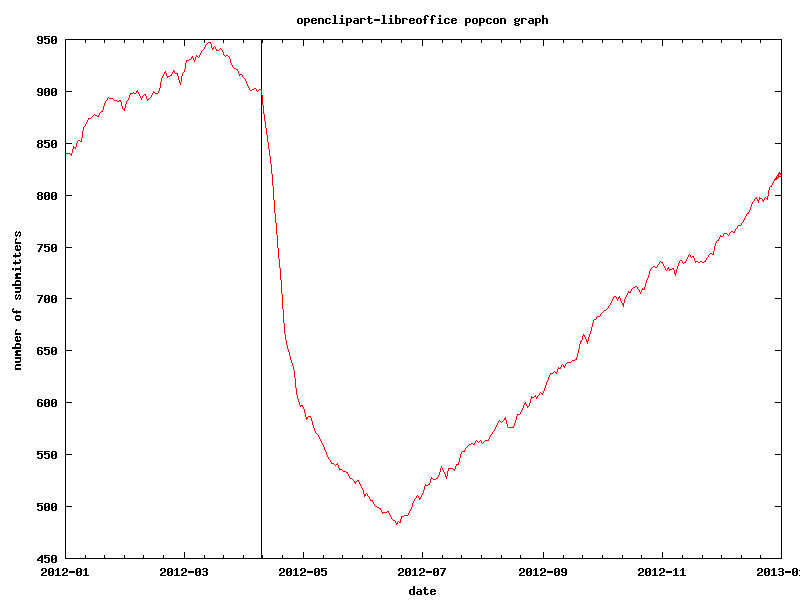
\includegraphics[width=0.8\linewidth]{figures/openclipart-libreoffice}
\end{center}
\end{frame}

\part{History}
\frame{\partpage}

\begin{frame}{Global goal}

\EEE{Analyze conflicts between packages}
\begin{itemize}
\item which packages can be installed
\item what packages conflit
\item conflict evolution
\item package migration
\end{itemize}

\end{frame}

\begin{frame}{Package installability}

List all packages which cannot be installed at all in a repository.
\texttt{debcheck}

Now, package \texttt{dose-distcheck}

Debian Weather (down?)
\url{http://edos.debian.net/weather/}

\url{http://qa.debian.org/debcheck.php}

Clear expectation: all packages should be installable

\end{frame}

\begin{frame}[fragile]{Co-installability}
Definition: a set of packages are co-installable if they can be install
together.

Package incompatibilities  are to be expected.
%
How do we visualize them?

See \url{http://coinst.irill.org/}
\end{frame}

\begin{frame}[fragile]{Co-installability graphs}
\begin{alltt}
coinst -root \EEE{iceweasel} -o graph.dot Packages_i386
\end{alltt}
\vspace{-2.5em}
\begin{center}
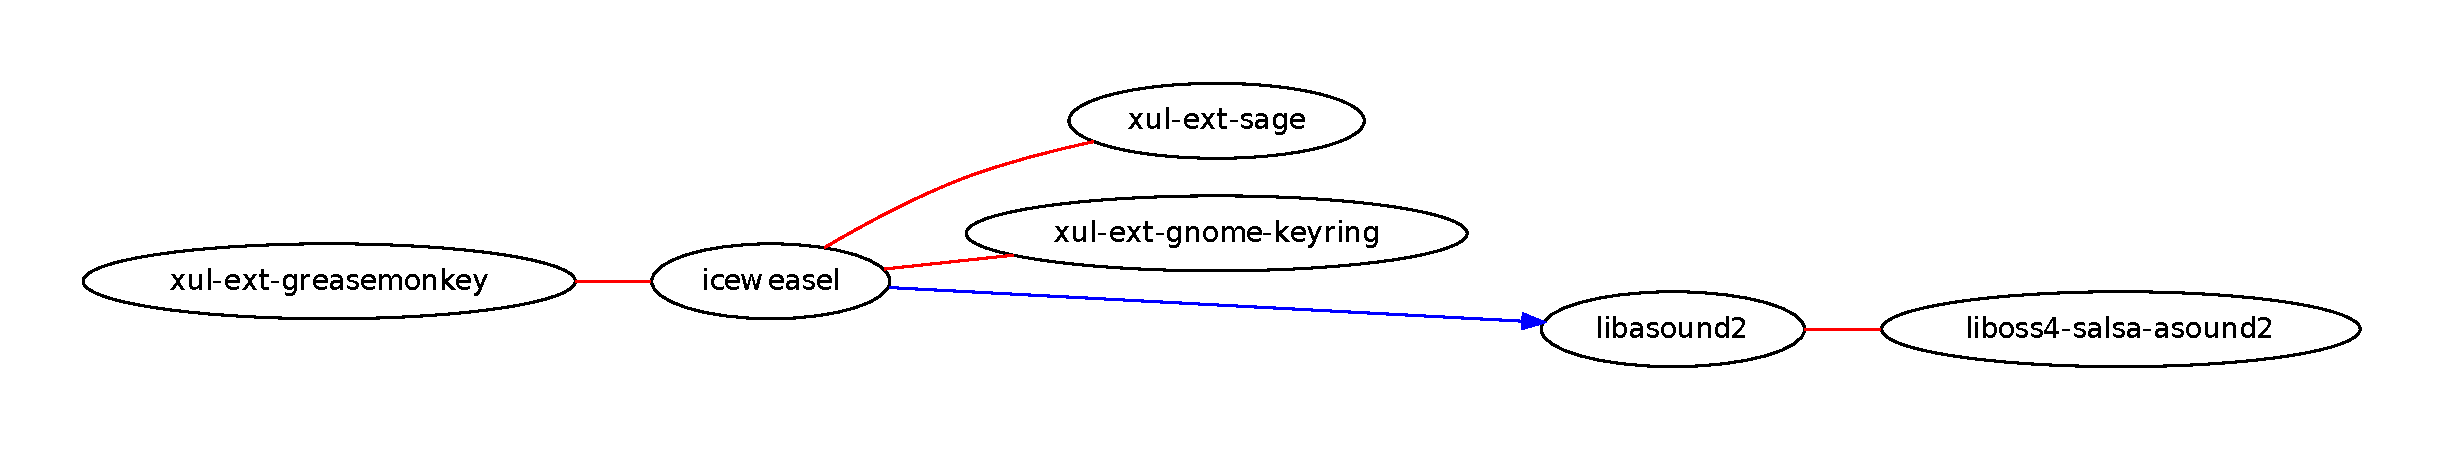
\includegraphics[width=\linewidth]{figures/iceweasel.pdf}
\end{center}
\vspace{-2em}
\begin{alltt}
coinst -root \EEE{kde-full} -o graph.dot Packages_i386
\end{alltt}
\vspace{-2.5em}
\begin{center}
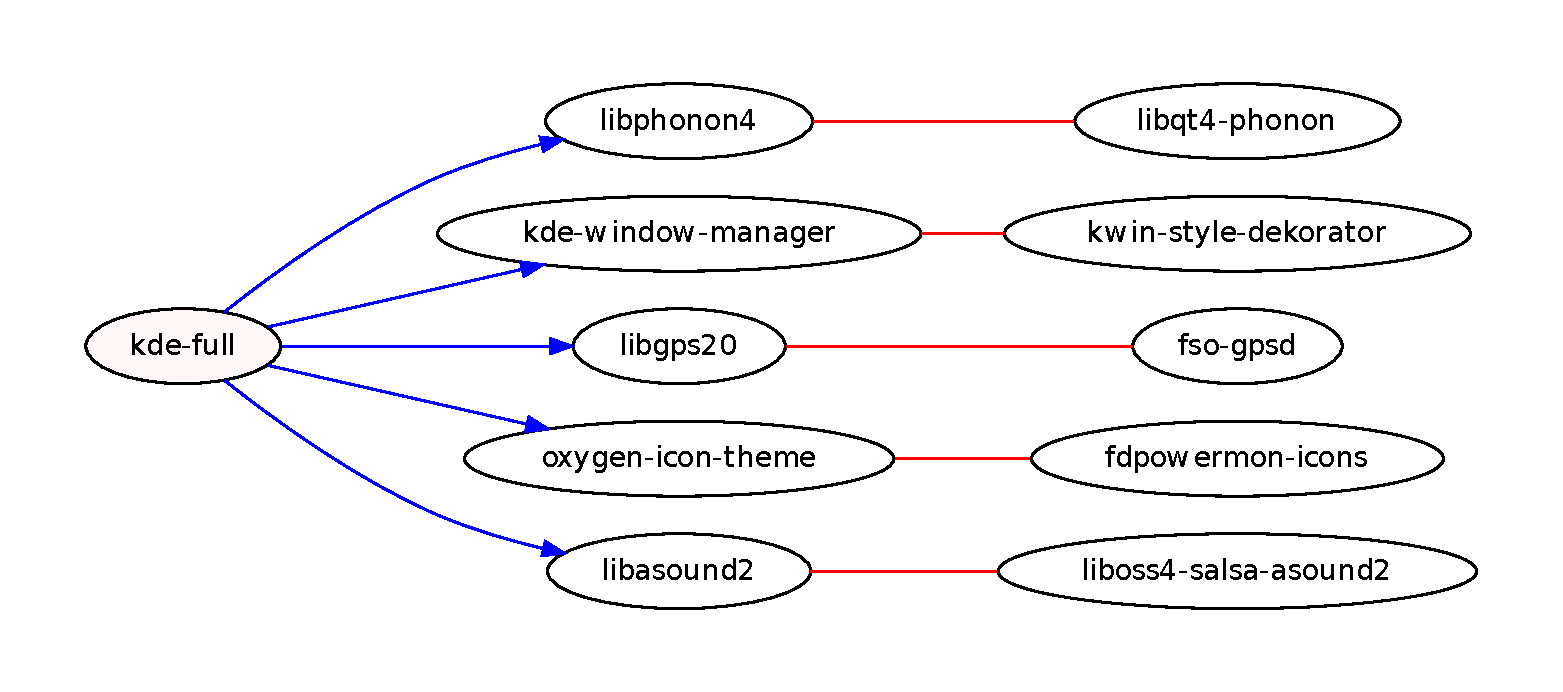
\includegraphics[width=0.65\linewidth]{figures/kde-full.pdf}
\end{center}
\end{frame}

\begin{frame}
\begin{center}
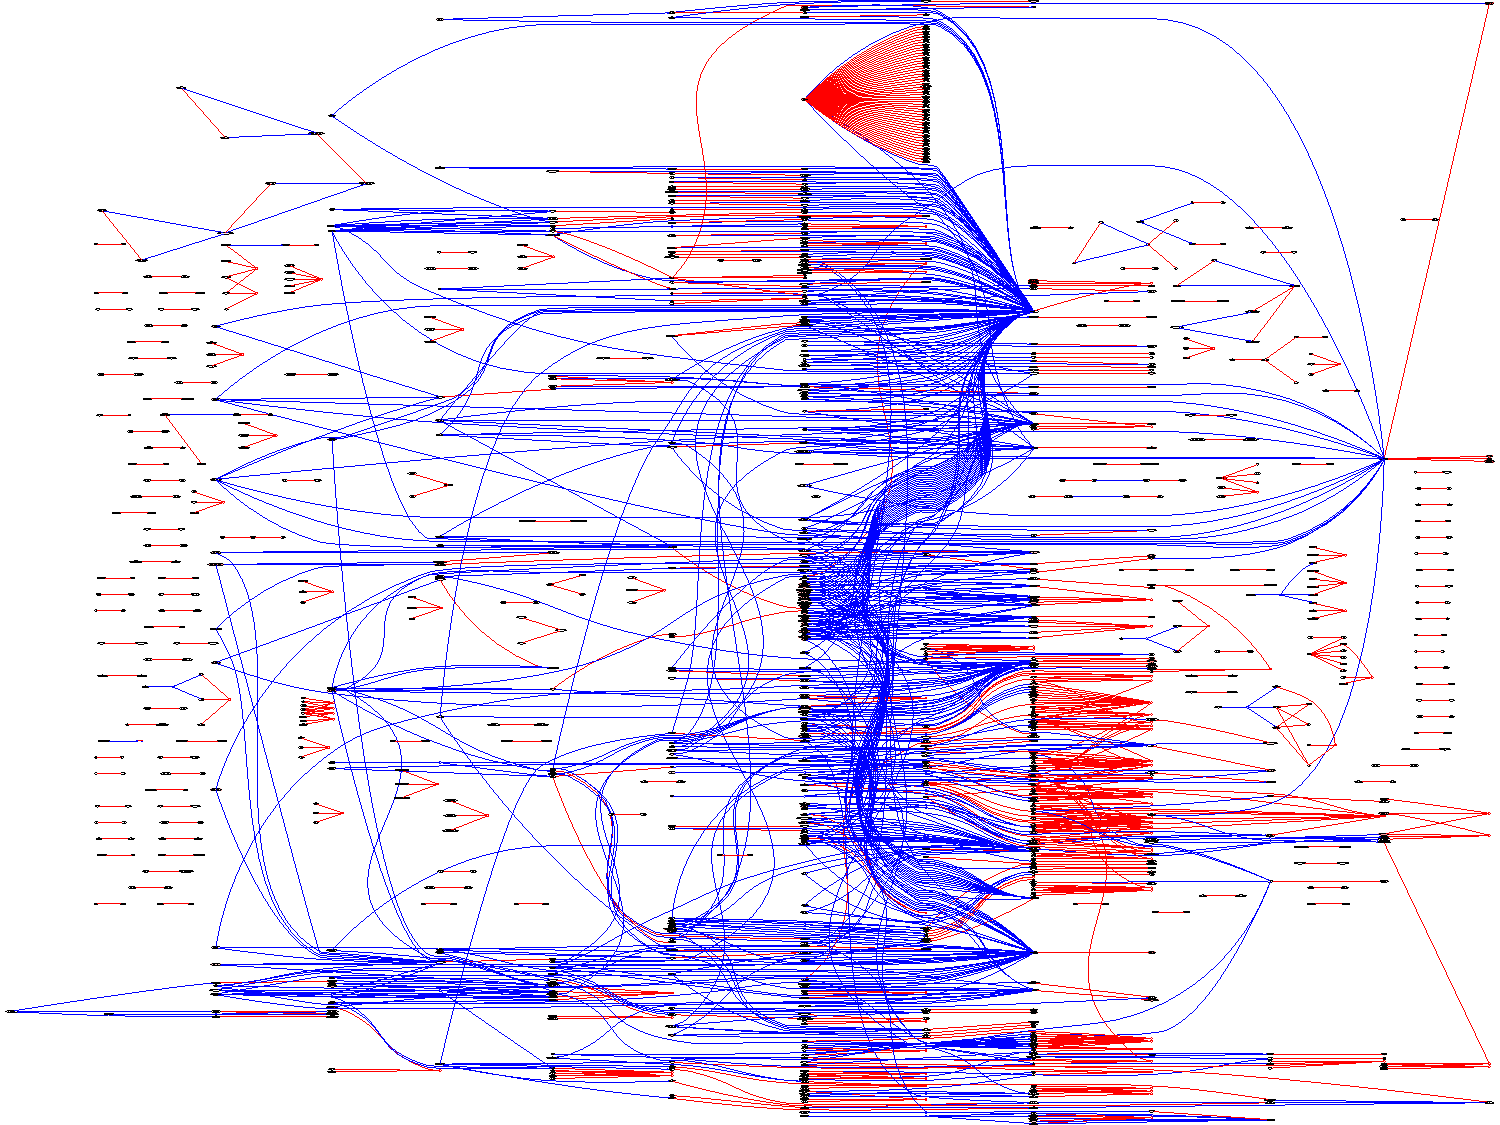
\includegraphics[width=\linewidth]{figures/flattened}
\end{center}
\end{frame}

\begin{frame}{Co-installability: algorithm}
\EEE{Key ideas}
\begin{itemize}
\item Transitive closures of package dependencies
\item Remove dependencies that can always be satisfied
\end{itemize}

\begin{center}
\begin{tabular}{@{}lrrrrrr@{}}
\toprule
& Before & After \\
\midrule
Packages & 28919 & 1038 \\
Dependencies & 124246 & 619 \\
Conflicts & 1146 & 985 \\
Median cone size & 38 & 1 \\
Avg. cone size & 66 & 1.7 \\
Max. cone size & 1134 & 15 \\
\midrule
Running time
& & 10.6 seconds
\\
\bottomrule
\end{tabular}
\end{center}

\end{frame}

\begin{frame}{Distribution evolution}
\url{http://coinst.irill.org/upgrades}

find new issues

present properly these issues (KDE example)

\begin{center}

\includegraphics{figures/libiodbc2}
\end{center}

\texttt{libiodbc2} is obsoletes

\end{frame}

\begin{frame}{Context}
\begin{center}

\includegraphics{figures/libiodbc2}
\end{center}
Depend on \texttt{libiodbc2} (about 380 package):
kcolorchooser kdesdk-misc kdevelop-php-docs blinken kdevelop
kmousetool ktorrent kalgebra konqueror klipper kchmviewer
mplayerthumbs libsmokekutils3 kjots ksshaskpass cantor
network-manager-kde kbattleship choqok kdesdk-dbg krusader-dbg
libkdegames-dev kmidimon klettres quassel-kde4 libakonadi-ruby
konq-plugins ktorrent-dbg kiriki plasma-widgets-workspace kvirc-dbg
konversation-dbg libkiten-dev kdm-gdmcompat plasma-netbook
libokular-ruby1.8 eqonomize kdenetwork-dbg libsmokeplasma3 kspread
lokalize korganizer parley kfourinline libsmokekde-dev kfind
kdepim-groupware ksnapshot libiodbc2-dev plasma-runners-addons
libsmokekdeui4-3 printer-applet ark kdeutils kover rocs kdesvn-dbg
kdevplatform-dev libkdepim4 ktron cantor-backend-sage kinfocenter
kjumpingcube kaddressbook kmymoney akonadiconsole cantor-backend-r
kmines kgoldrunner partitionmanager libsublime-dev korundum4
kphotoalbum kplayer
\ldots

\end{frame}

\part{Comigrate}
\frame{\partpage}

\begin{frame}{Applications}
\begin{itemize}
\item interactively investigate migration issues
\item report of issues preventing package migration
\end{itemize}
\end{frame}

\begin{frame}{Tool architecture}

\begin{itemize}
\item
 use Boolean solver to generate a tentative solution
  (extremely efficient)
\item
 check for (co-)installability issues;
  analyse these issues to generate new Boolean constraints
  (typically: if these packages do not migrate, this package cannot migrate)
\item iterate...
\end{itemize}
\end{frame}

\begin{frame}{Performance}

XXX Context

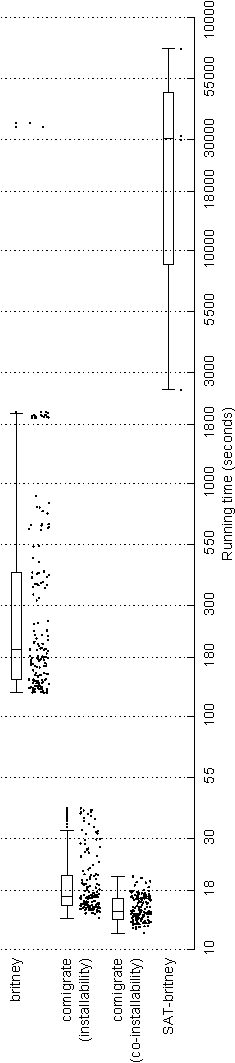
\includegraphics[height=\linewidth,angle=-90]{figures/performance.pdf}
\end{frame}

\begin{frame}{Ressources}
Tool: \url{http://coinst.irill.org/comigrate}
(Debian packages forthcoming?)

Packages \texttt{dose-distcheck}, \texttt{coinst}, and
\texttt{coinst-viewer} in Debian

\url{https://github.com/vouillon/coinst}

Daily report:
\url{coinst.irill.org/report}
\end{frame}

\end{document}
